\documentclass[tilz, border=10pt]{standalone}

\usepackage{tikz}
\usetikzlibrary{arrows, automata}

\tikzset{
    every state/.style={fill=orange, draw=none, text=white},
    accepting/.style={draw, green!50!black, text=white, accepting by double},
    initial/.style={fill=red, text=white, initial by arrow, initial text=start, initial distance=20pt}
}

\begin{document}
    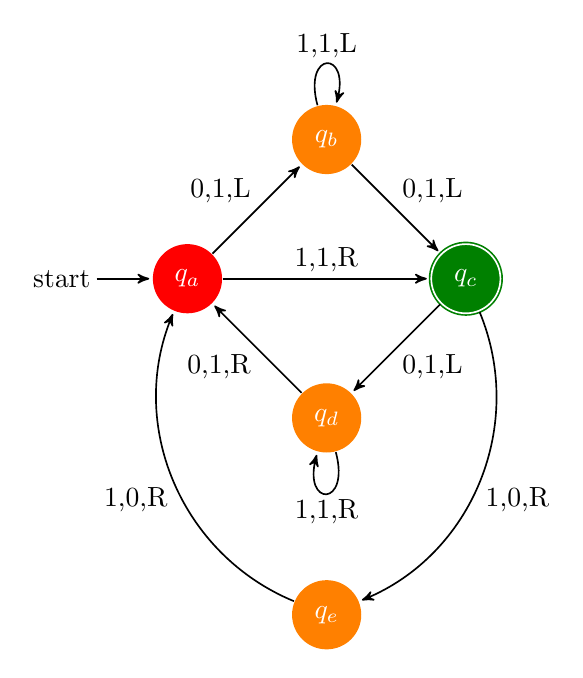
\begin{tikzpicture}[
        ->, >=stealth', shorten >=1pt, semithick,
        auto, node distance=2.5cm,
        inner sep=2pt, bend angle=45
    ]
        \node[state, initial] (A) {$q_a$};
        \node[state] (B) [above right of=A] {$q_b$};
        \node[state, accepting] (C) [below right of=B] {$q_c$};
        \node[state] (D) [below right of=A] {$q_d$};
        \node[state] (E) [below of=D] {$q_e$};
        
    
        \path (A) edge node {0,1,L} (B)
                  edge node {1,1,R} (C)
              (B) edge[loop above] node {1,1,L} ()
                  edge node {0,1,L} (C)
              (C) edge node {0,1,L} (D)
                  edge[bend left] node {1,0,R} (E)
              (D) edge[loop below] node {1,1,R} ()
                  edge node {0,1,R} (A)
              (E) edge[bend left] node {1,0,R} (A);
    \end{tikzpicture}
\end{document}